\section{A Theory for the Hydrogen Atom}

\makelabheader %(Space for student name, etc., defined in master.tex)

\textbf{Objective}

To use a numerical technique to solve the Schroedinger equation for the hydrogen atom,
compare calculations with spectroscopic measurements from hydrogen,
 and explore
the implications of the quantum theory especially the quantization of energy
in bound systems.

\textbf{Apparatus}

\begin{itemize}

\item {\it Schr\"odinger Shooter} software

\item Results from previous measurements of hydrogen energy transitions.

\end{itemize}

\textbf{Overview}

Quantum mechanics is the theoretical structure used to make sense of the atomic and sub-atomic
world. 
It is based on a small set of assumptions and a lot of associated mathematics.

\begin{center}
\bf The Postulates of Quantum Mechanics
\end{center}

\begin{enumerate}

\item The quantum state of a particle is characterized by a wave function  
$\Psi(\vec r,t)$, which contains all the information about the system an observer can 
possibly obtain.
The square of the magnitude of the wave function $|\Psi (\vec r,t)|^2$ 
is interpreted as a probability or probability density for the particle's presence. 

\item The things we measure ({\it e.g.} energy, momentum) are called observables. 
Each observable has a corresponding mathematical object called an operator 
that does `something' to the wave function $\Psi(\vec r,t)$.
The radial dependence of the wave function $\Psi(\vec r,t)$ is governed by
the energy operator which generates a famous expression called the
Schr\"odinger equation.
\begin{equation}
-\frac{\hbar^2}{2 m}\left ( \frac{d^2}{d r^2} +  
   \frac{L^2}{2 m r^2} \right ) \Psi(r) + U \Psi(r) = E  \Psi(r)
\end{equation}
Ultimately, the success of this approach will depend on how the theoretical
results we generate from solving the Schr\"odinger equation compare with
our measurements.

\end{enumerate}

\noindent We will focus on these postulates in this laboratory and in particular
on understanding and solving Equation 1, the Schr\"odinger equation.

\textbf{Activity 1: Energy in Three Dimensions}


Consider a particular form of the total
mechanical energy of a particle in three dimensions
\begin{equation}
E = \frac{1}{2} m \vec v \cdot \vec v + V(\vec r) = 
   \frac{1}{2} m (v_x^2 + v_y^2 + v_z^2) + V(\vec r) = 
   \frac{1}{2} m v^2 + V(\vec r) 
\end{equation}
where $m$ is the particle's mass, $\vec v$ is its
velocity, and  $V(\vec r)$ is the potential energy of the particle
and depends only on the particle's position.
We have used the definition of the momentum $\vec p = m \vec v$.
The potential energy between the electron and proton in a hydrogen atom is 
the Coulomb potential so
\begin{equation}
V(\vec r) = k_e \frac{q_1 q_2}{r} =  
   - k_e \frac{e^2}{r} 
\end{equation}
where we have used the known proton and electron charges.

If we have an electron in the vicinity of a proton ({\it i.e.} a hydrogen atom), then
it is convenient to rewrite the kinetic energy part of Equation 2 in polar coordinates.
The proton, electron and the electron's velocity vector 
form a plane where we can describe the velocity in terms
of a radial component and an angular one
\begin{equation}
\vec v = v_r \hat r + v_t \hat \theta
\end{equation}
where $\hat r$ points radially along a line from the origin to the electron's position
and $\hat \theta$ is perpendicular to $\hat r$ and points so counter-clockwise rotations
are positive.

(a) Get an expression for $v^2$ in terms of
$v_r$ and $v_t$ and substitute your result in the energy equation (Equation 2).
\vskip 2.0cm

(b) We can now define the momentum associated with  the radial motion
as $\vec p_r = m\vec v_r$
and the momentum associated with the angular motion $L = mrv_t$.
The angular momentum $L$ is a constant of the motion so it is unchanging.
Rewrite your energy equation in terms of $p_r$, $L$, $r$, and any other constants.
Include the explicit version of the potential in Equation 3.
\vskip 2.0cm

(c) You should have found in part 1.b that the three-dimensional
energy of a particle in a Coulomb field can be written as
\begin{equation}
E = \frac{p_r^2}{2m} + \frac{L^2}{2mr^2} - k_e\frac{e^2}{r}
\end{equation}
where $L$ is a constant so the energy only depends on $r$ and $p_r$.
Note the similarities with the forms of the Schr\"odinger equation in Equation 1.
Make a sketch of the potential energy as a function of $r$.
What are the limiting values of the potential?
\vskip 3.0cm

(d) The angular momentum $L$ is a constant of the motion so the last two terms in 
Equation 5 can be treated as a single `effective' potential that governs the radial motion
of particles.
Make a sketch of those last two terms as a function of $r$ for constant $L$.
How is your figure different from the one in 1.c?
\vskip 3.0cm

\newpage

(e) Since the energy is constant you can draw it on your previous sketch as a flat, straight
line. We are considering bound states (the hydrogen atom) so $E < 0$.
Draw an energy line for a bound state on your previous sketch.
Does your energy `curve' intersect the effective potential curve anywhere?
For a classical particle like a ball rolling on a hill or a satellite orbiting the
Earth,
what happens at this intersection?
Describe the motion of a classical particle in this potential.
What restrictions are there on the energy $E$ of a classical particle?
\vskip 3.0cm

\textbf{Activity 2: Quantum Predictions}

(a) What do you expect the wave function of the electron in a hydrogen atom to look like?
Copy your drawing from part 1.d and add
a sketch of your expectation for the hydrogen atom wave function on the same graph. 
Consider what happens
as the effective potential changes with $r$.
\vskip 4.0cm

(b) What happens to your wave function as the energy increases?
Make another copy here of the graph of the effective potential energy that you made in 2.a.
Draw an energy curve for a higher energy state than your previous one.
Now sketch the new, higher-energy wave function.
How is it different from the curve you made in 2.a?
\vskip 4.0cm

\textbf{Activity 3: Solving the Schr\"odinger Equation}

(a) We are now ready to start solving the Schr\"odinger Equation.
Go first to the {\tt All Programs} menu, then
to {\tt Physics Applications} and click on {\tt Schr\"odinger Shooter}.
You will see the {\tt Schr\"odinger Shooter} window like the one in the next figure.
If you don't see this window, consult your instructor.
\begin{figure}[hbt]
\begin{center}
\includegraphics[width=6.0in]{solveSE/shooter1b.eps}
\caption{Initial panel for {\it Schr\"odinger Shooter}}
\index{color page}
\end{center}
\end{figure}

(b) The first step is to select a potential energy function.
Click on {\tt File} and go to {\tt New Potential Energy Function}.
Select the potential energy function most appropriate for the hydrogen atom.
Next select the charge of the atomic nucleus by entering that value in the 
box labeled {\tt Z:} in units of the electronic charge $e$.
Set the quantum number of the angular momentum to zero in the box
labeled {\tt L:}.
Use the second menu button from the left-hand side 
at the bottom of the {\tt Schr\"odinger Shooter}
window to choose {\tt Normalized} wave functions (it should be labeled {\tt Not Normalized}
when you start the program).
This last choice makes it easier to compare wave functions for different quantum numbers.
Last, set the initial value of the energy to -1.5 in the box labeled 
{\tt Energy (Rydbergs):} and hit return.
The conversion between eV and rydbergs is $\rm 13.605 6923(12)~ eV/rydberg$.
The number in parentheses is the uncertainty on the last two digits in the
experimental value.
At this point you should see curves in both of the panels of the 
{\tt Schr\"odinger Shooter} window.
If you don't, consult your instructor.

(c) You should see several curves in the upper panel.
What quantities do the blue, red, yellow, and green curves represent?
Use the legend in the lower right portion of the {\tt Schr\"odinger Shooter}
window.
Record them here.
\vspace{2.5cm}

(d) You can now adjust the energy of the electron in the field of the proton to find 
the energy levels of hydrogen.
There are three ways to change this energy.
There is a slide on the left-hand side of the {\tt Schr\"odinger Shooter} window.
Click and drag the slide to change the energy and read the value
in the box labeled {\tt Energy(Rydbergs)} located near the top of the 
{\tt Schr\"odinger Shooter} window.
You can also enter the energy in the same box
labeled {\tt Energy(Rydbergs):} as you did in part 3.b.
Last, to the right of this last box there are buttons labeled
{\tt Adjust Energy:} that will increase or decrease the energy and change the step size.

(e) Tune the energy to find lowest five energy levels in your hydrogen atom by obtaining
physically acceptable wave functions.
You may need to increase the horizontal range to view the full wave function.
You can do this by increasing the value in the box labeled {\tt Cutoff:} at the
bottom of the {\tt Schr\"odinger Shooter} window.
If you increase the horizontal scale, then increase the next box labeled
{\tt Count:} (next to the {\tt Cutoff} box) by the same ratio.
In other words, if you double the cutoff, then double the count.
This last parameter controls the stepsize used in the numerical integration of
the Schr\"odinger equation.
What does the wave function look like when you have found the correct energy level?
What postulate did you exploit to find the correct solutions?
How does the radial wave function change as the energy increases?
Record you values for each of the energy levels below.
\vspace{5.0cm}

\textbf{Activity 4: Analysis and Comparison with Previous Data}

(a) Enter the values you found for the energies in an {\it Excel} spreadsheet
and convert the values to eV.
Use the scale below to make an energy level diagram for hydrogen.

\vspace{0.25in}

\hspace{1.0cm}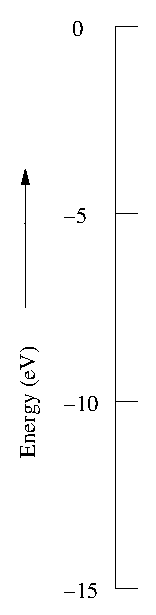
\includegraphics{solveSE/energyLevels.eps}

\vspace{0.75in}

\newpage

(b) In the lab entitled {\it Optical Spectrum of Hydrogen}
you measured and identified transitions in hydrogen between different
principle quantum levels.
Using the results in part 4.a calculate the energies of the 
same transitions and the wavelength of the emitted photon.
Record your results below.
\vspace{4.0cm}

(c) Compare your measured results from the {\it Optical Spectrum of Hydrogen}
with the predictions of your model in part 4.b.
Calculate the percentage difference for each transition.
Does your model agree with the data?
Be quantitative in your answer.
\vspace{3.0cm}


\textbf{Activity 5: The Meaning of Quantum Theory}

(a) For one of your hydrogen energy states, change the angular momentum of the
quantum state by setting $L=1$ in the box labeled {\tt L:}.
How does the radial wave function change?
How much does the energy change?
Do the same thing with the next higher energy state.
Can you jump to any conclusions about the effect of angular momentum on the energy
of a quantum state in hydrogen?
\vspace{2.0cm}

(b) Return to the questions in Activity 2 and examine your predictions.
How did you do?
Correct any statements that you now find are wrong.
\vspace{2.0cm}

(c) What requirement or postulate forces us to choose particular energy states
({\it i.e.} what causes energy quantization)?
\vspace{2.0cm}

\newpage

(d) Reconsider a variation of one of the questions in part 1.e.
In that question you were asked to describe the motion of a classical particle
like a satellite orbiting the Earth.
Describe the motion of a quantum particle in the hydrogen atom potential.
\vspace{3.0cm}

\textbf{Homework}

\begin{enumerate}

\item An atom (not a hydrogen atom) absorbs a photon whose frequency is
$f = 6.2\times 10^{14}~Hz$.
How much does the energy of the atom increase?

\item What is the energy of the hydrogen atom  electron whose probability density
is represented by the dot plot shown below? 
What minimum energy is needed to remove this electron from the atom?
\begin{figure}[hbt]
\begin{center}
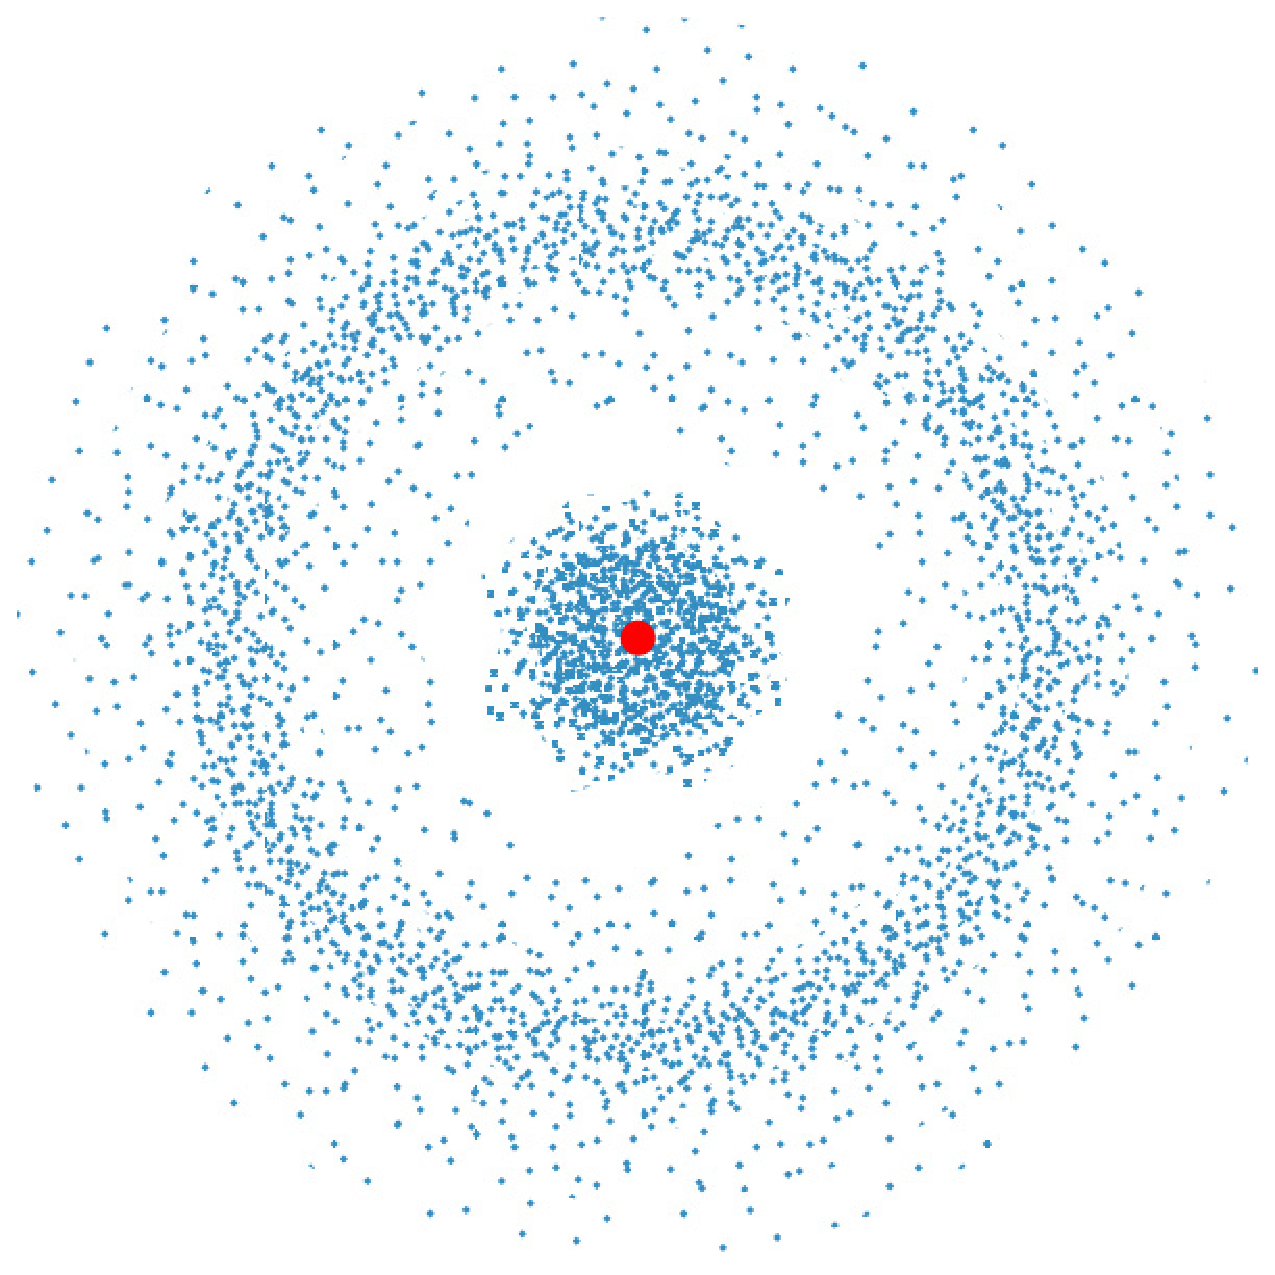
\includegraphics[height=1.5in]{solveSE/hwfig2.eps}
\index{color page}
\end{center}
\end{figure}

\item What are the energy and wavelength of a photon emitted when a hydrogen atom
undergoes a transition from the $n=3$ state to the $n=1$ state?

\item What is the wavelength of the least energetic photon emitted in the Lyman
series (where $n_f = 1$) of the hydrogen atom spectrum lines?

\item What is the series limit for the Lyman series (where $n_f = 1$)?

\end{enumerate}
